\exer{Numérotation des points d'un quadrillage}
\setcounter{numques}{0}

%\begin{flushright}
%\footnotesize{D'après Jean-Pierre Becirspahic.}
%\end{flushright}



On démontre que l'ensemble $\mathbb{N}\times \mathbb{N}$ est dénombrable en numérotant chaque couple $(x,y)\in\mathbb{N}^2$ suivant le procédé suggéré par la figure ci-dessous.

\begin{center}
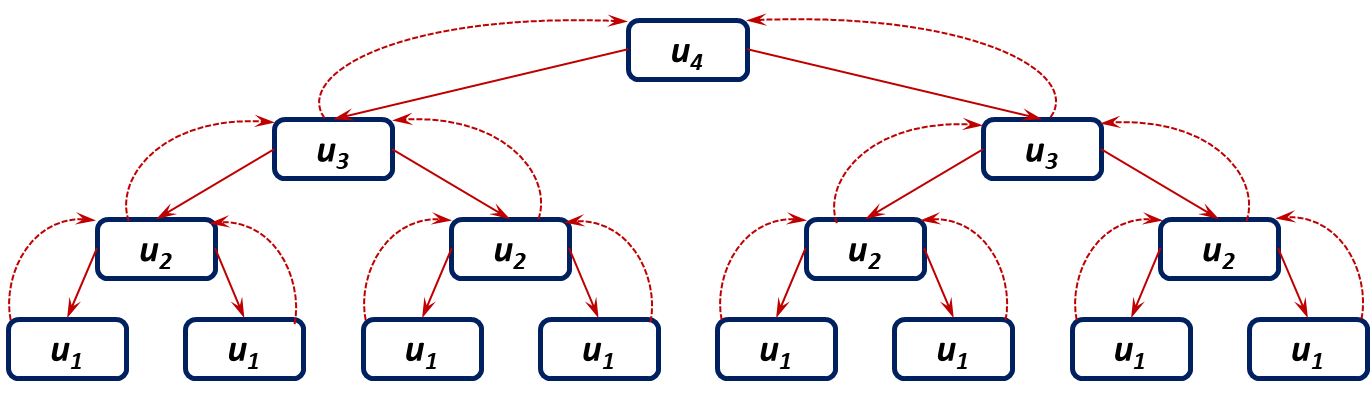
\includegraphics[width=.2\linewidth]{images/fig_01}
\end{center}

\question{Rédiger une fonction récursive \texttt{numerote(n:int) -> int} qui retourne le numéro du point de coordonnées $(x,y)$.}
\ifprof
\begin{lstlisting}
def numerote(x, y):
    if x == 0 and y == 0:
        return 0
    if y > 0:
        return 1 + numerote(x+1, y-1)
    return 1 + numerote(0, x-1)
\end{lstlisting}
\else

\fi

\question{Rédiger la fonction \texttt{reciproque(n:int) -> tuple}, là encore de façon récursive}.
\ifprof
\begin{lstlisting}
def reciproque(n):
    if n == 0:
        return (0, 0)
    (x, y) = reciproque(n-1)
    if x > 0:
        return (x-1, y+1)
    return (y+1, 0)
\end{lstlisting}
\else

\fi
